\documentclass[11pt,a4paper]{article}

\usepackage[margin=1.85cm]{geometry}
\usepackage[T1]{fontenc}
\usepackage[utf8]{inputenc}
\usepackage{lmodern}
\usepackage{microtype}
\usepackage{amsmath}
\usepackage{graphicx}
\usepackage{booktabs}
\usepackage{tabularx}
\usepackage{array}
\usepackage{enumitem}
\usepackage{xcolor}
\usepackage{hyperref}
\usepackage{float}

\graphicspath{{../assets/}}
\hypersetup{colorlinks=true,linkcolor=blue,urlcolor=blue,citecolor=blue,hypertexnames=false}
\setlist[itemize]{leftmargin=1.2em,itemsep=0.05em,topsep=0.1em}
\setlist[enumerate]{leftmargin=1.35em,itemsep=0.05em,topsep=0.1em}
\renewcommand{\arraystretch}{1.08}
\setlength{\parindent}{0pt}
\setlength{\parskip}{0.28em}
\emergencystretch=3em
\Urlmuskip=0mu plus 1mu\relax
\newcommand{\code}[1]{\texttt{\detokenize{#1}}}

\title{\vspace{-1.1cm}CyberSecIntel\\P2 Final Delivery\\Trusted Zone, Exploitation Zone, Consumption, and Governance}
\author{D\'idac Cayuela and Sindri Masson\\Big Data Management -- Universitat Politecnica de Catalunya}
\date{May 2026}

\begin{document}
\maketitle
\vspace{-0.85cm}

\section{Instructions}

CyberSecIntel is a cybersecurity data platform for small SOC workflows. P1 implemented ingestion and a governed Landing/Silver lakehouse: public vulnerability feeds, IOC feeds, CTU-13 PCAP artifacts, Suricata replay outputs, and Kafka topics are stored in MinIO and Delta Lake. P2 completes the architecture required by the statement: Trusted Zone, Exploitation Zone, downstream consumption, and governance.

\textbf{Run order.}
\begin{enumerate}
  \item Copy configuration: \code{cp .env.example .env}; optional keys are \code{NVD_API_KEY}, \code{ABUSE_CH_API_KEY}, and \code{SHODAN_API_KEY}.
  \item Start infrastructure: \code{docker compose build airflow-webserver}; \code{docker compose up -d minio zookeeper kafka postgres}; \code{docker compose run --rm airflow-init}; \code{docker compose up -d airflow-webserver airflow-scheduler}.
  \item Run P1 ingestion: trigger \code{cybersecintel_api_expansion_ingestion}; optionally run \code{cybersecintel_dataset_artifact_ingestion} and \code{cybersecintel_pcap_replay}.
  \item Run P2: trigger \code{cybersecintel_trusted_zone}, then \code{cybersecintel_exploitation_zone}, then \code{cybersecintel_consumption_exports}.
\end{enumerate}

The P2 stages can also be executed locally after P1 Delta tables exist:
\begin{verbatim}
python -m trusted.run_trusted
python -m exploitation.run_exploitation --warm
python -m consumption.run_exports
\end{verbatim}
The outputs are inspected in MinIO buckets \code{s3://trusted/} and \code{s3://exploitation/}, plus local files under \code{consumption/outputs/}.

\textbf{Submission evidence.} The final archive contains the source code, report source, generated PDF, tests, Docker/Airflow definitions, the trained ML model artifact, and generated consumption files. The verification run used the same Docker Compose stack as the coursework demo, so the evidence is not limited to isolated unit tests. The key observed P2 outputs were: 11 Trusted lineage rows, 44 Trusted quality-metric rows, 6 exploitation catalog products, 11 exploitation lineage rows, 16 exploitation quality-metric rows, 50 CVE prioritization rows, 10664 ML anomaly records on the replay dataset, and all five consumption files.

\section{Architecture Design}

The final architecture follows Option 1 from the P2 statement: extend the P1 lakehouse instead of adding several specialized databases. This is appropriate because the project has heterogeneous cybersecurity sources but moderate volume, and the main need is reproducible movement through zones, not ultra-low-latency OLAP serving. MinIO remains the object store and Delta Lake remains the table format for all checkpoints.

\begin{figure}[H]
  \centering
  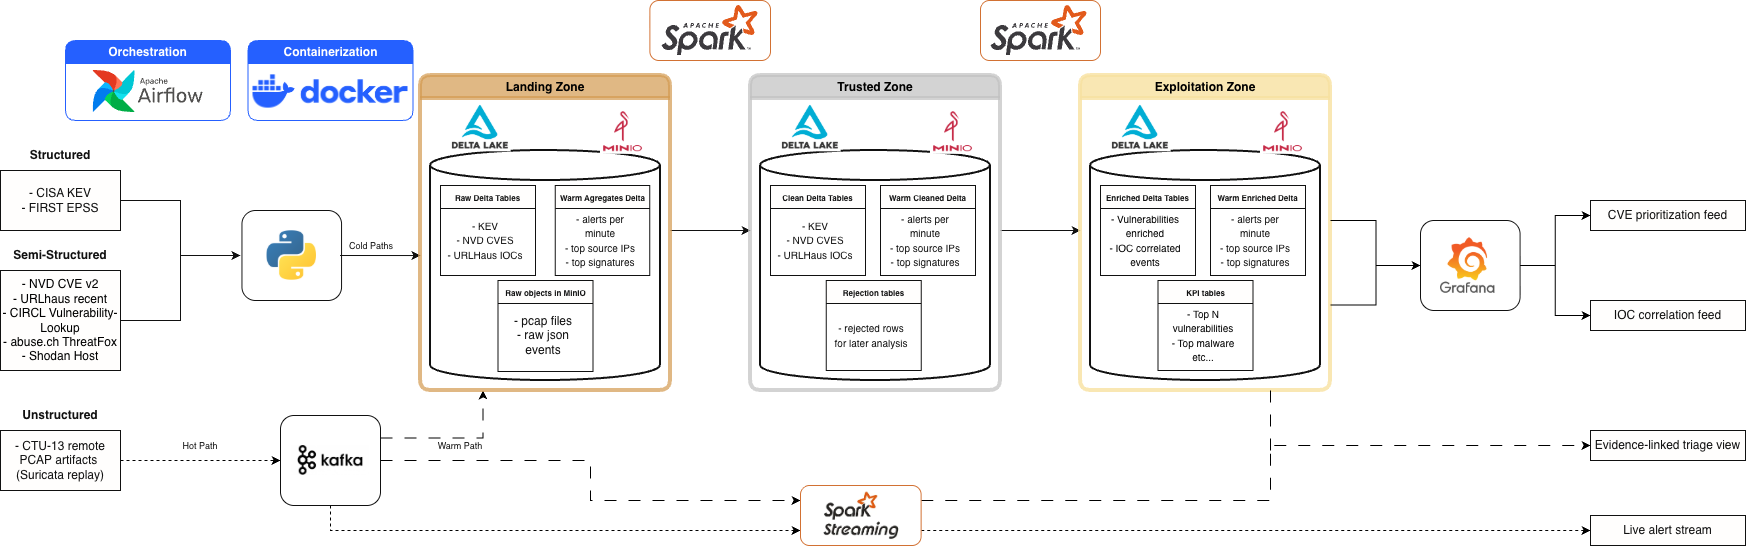
\includegraphics[width=\textwidth,height=0.46\textheight,keepaspectratio]{BDM_P2.drawio.png}
  \caption{Final P2 architecture. P1 feeds Landing/Silver; P2 adds Trusted, Exploitation, Consumption, and Governance checkpoints.}
\end{figure}

\begin{tabularx}{\textwidth}{>{\raggedright\arraybackslash}p{2.8cm}X}
\toprule
\textbf{Stage} & \textbf{Implemented role}\\
\midrule
Landing/Silver & P1 raw MinIO prefixes and Delta tables: KEV, NVD, EPSS, URLhaus, CIRCL, ThreatFox, optional Shodan, PCAP catalogs, replay runs, Suricata events, and IDS alerts.\\
Trusted & \code{trusted/} package reads \code{s3://deltalake/}, performs information-preserving cleaning, writes cleaned tables and rejected-row tables to \code{s3://trusted/}.\\
Exploitation & \code{exploitation/} package writes analyst-ready Delta assets to \code{s3://exploitation/}: CVE enrichment, network events, IOC correlations, anomaly flags, warm enriched alerts, and KPIs.\\
Consumption & \code{consumption/} package exports CSV, JSON, and an HTML SOC dashboard from exploitation assets. Kafka topics remain available for live event inspection.\\
Governance & \code{governance/} package creates data product catalog, lineage records, and quality metrics for Trusted, Exploitation, and Consumption runs.\\
\bottomrule
\end{tabularx}

The cold path is Airflow-orchestrated batch movement through P1 ingestion, Trusted cleaning, Exploitation materialization, and file exports. The warm path uses the P1 \code{ids.alerts} Kafka topic and a bounded consumer that enriches alerts against \code{vuln_enriched}; it is bounded so the Airflow task terminates reliably in a coursework demonstration. The hot path remains the P1 \code{suricata.events} topic, where raw replay events are already normalized and should not be delayed by extra transformations.

\subsection{Why the same lakehouse stack is kept}

The P2 statement offers two implementation directions: extending the current architecture or moving parts of the pipeline to specialized databases. We keep the first option. This decision is not a simplification of the data-management problem; it is a deliberate fit to the workload. The project's largest operational dataset is replay-derived network telemetry, while the vulnerability and IOC feeds are moderate in size. MinIO and Delta Lake provide clear zone separation, ACID table commits, schema evolution, reproducible overwrite checkpoints, and direct Python access without operating extra services. Adding ClickHouse, MongoDB, Milvus, or Grafana would make the architecture broader, but not more reliable for the final marking criteria unless those services were deeply integrated and validated.

The implementation therefore treats each zone as a managed checkpoint:
\begin{itemize}
  \item \textbf{Landing/Silver}: source-native evidence and queryable P1 Delta tables.
  \item \textbf{Trusted}: cleaned, deduplicated, auditable records plus rejected-row tables.
  \item \textbf{Exploitation}: denormalized analytical products, KPIs, ML predictions, and governance metadata.
  \item \textbf{Consumption}: files and dashboard that prove analysts can consume the exploitation assets.
\end{itemize}

This structure matches the P1 principle of preserving raw evidence first and modelling later. It also satisfies the P2 requirement that each zone has separate storage after its respective transformations.

\section{Trusted Zone}

The Trusted Zone applies the P2 statement's information-preserving rule: clean representational problems without encoding downstream modelling assumptions. The implementation is in \code{trusted/cleaning.py} and \code{trusted/run_trusted.py}.

\begin{tabularx}{\textwidth}{>{\raggedright\arraybackslash}p{2.8cm}X}
\toprule
\textbf{Source family} & \textbf{Trusted transformations}\\
\midrule
Structured & KEV and EPSS: CVE normalization, date parsing, numeric casting, EPSS range warnings, mandatory-field checks, and deduplication by natural key.\\
Semi-structured & NVD, CIRCL, URLhaus, ThreatFox, and Shodan: stable helper fields, CVE/indicator normalization, URL or score warnings, JSON-safe nested values, and deduplication.\\
Network and PCAP-derived & PCAP artifacts, replay runs, Suricata events, and IDS alerts: timestamp validation, integer casting, ingest-date preservation, integrity flags, and event deduplication.\\
\bottomrule
\end{tabularx}

Rows with missing mandatory fields and duplicate keys are written to \code{rejected_*} Delta tables rather than silently discarded. Rows with suspicious but still usable values receive \code{_quality_warn} and \code{_quality_reasons}. This gives downstream tasks cleaner tables while preserving auditability and avoiding lossy deletion.

Each Trusted run also writes \code{governance_lineage} and \code{governance_quality_metrics} in the Trusted bucket. The metrics record rows read, rows written, rows rejected, and warning counts per source table.

\subsection{Trusted schemas and quality policy}

The Trusted Zone is intentionally conservative. CVE-like fields are uppercased and normalized into \code{cve_id}; dates are parsed into ISO formats; numeric fields such as EPSS, CVSS, severity, ports, file size, and replay counters are cast when possible; URLhaus URLs are checked for a valid HTTP(S) prefix; and network timestamps are normalized. These changes improve representational quality without changing the analytical meaning of the records.

The key quality policy is that a bad value should not automatically erase a security signal. A CVE record with an out-of-range EPSS value is still useful for traceability, so it is retained with warning flags. A row missing the natural key needed for downstream joins is not safe for analytical products, so it is moved to the rejected table with its original JSON payload and rejection reason. This distinction is important for grading: the cleaning task is not merely a technical filter, but a governed data-quality decision.

\section{Exploitation Zone}

The Exploitation Zone organizes data as SOC-facing products rather than raw source copies. The implementation is in \code{exploitation/analytics.py}, \code{exploitation/warm_path.py}, and \code{exploitation/run_exploitation.py}.

\begin{tabularx}{\textwidth}{>{\raggedright\arraybackslash}p{3.1cm}X}
\toprule
\textbf{Asset} & \textbf{Purpose}\\
\midrule
\code{vuln_enriched} & Wide CVE table joining KEV, NVD, EPSS, and CIRCL by normalized \code{cve_id}. It includes KEV status, dates, descriptions, EPSS, CVSS, reference counts, and \code{vuln_priority_score}.\\
\code{network_events} & Unified IDS and Suricata schema with timestamp, event type, source/destination, ports, protocol, signature, severity, category, and origin source.\\
\code{ioc_correlations} & Matches observed network IPs, URLs, and hostnames against ThreatFox, URLhaus, and Shodan indicators where possible.\\
\code{anomaly_flags} & ML anomaly predictions over network events. The model learns robust baselines from severity, source/destination ports, source/destination frequency, signature frequency, and remote-access-port indicators, then writes anomalous events with score, threshold, label, and reasons.\\
\code{warm_enriched_alerts} & Bounded Kafka warm-path output: IDS alerts enriched with CVE priority and severity context when the alert mentions a CVE.\\
KPI tables & Top vulnerabilities, daily alert counts, top signatures, top source IPs, and recent KEV additions.\\
\bottomrule
\end{tabularx}

The vulnerability priority score follows the design from P2.1:
\[
\textit{priority} = \textit{epss\_score} \times (1.5 \text{ if KEV-listed else } 1.0) \times \frac{\textit{cvss\_v3\_score}}{10}
\]
If CVSS is unavailable for a CVE in the current source snapshot, the score still remains usable through EPSS and KEV. This gives patch teams a ranked list even when public data sources differ in completeness.

\subsection{ML anomaly prediction}

P2.1 proposed an Isolation Forest anomaly feed. The final implementation keeps that promise at the level that is most robust for this local stack: a dependency-free unsupervised anomaly model trained from the exploitation network events. The model is implemented in \code{exploitation/ml_anomaly.py}. It extracts a feature vector per event:
\begin{itemize}
  \item severity;
  \item source and destination ports;
  \item source-IP, destination-IP, and signature frequencies in the current event population;
  \item a binary indicator for suspicious remote-access/control ports such as 23, 2323, 3389, 4444, and 5900.
\end{itemize}

The training stage learns robust medians and median absolute deviations for each feature and sets a 95th-percentile anomaly threshold over the training distribution. The inference stage scores each event against that learned baseline and emits records whose score crosses the threshold or whose feature pattern contains high-risk security indicators. Each output row includes \code{ml_score}, \code{ml_threshold}, \code{prediction_label}, and human-readable \code{anomaly_reasons}. This is a real trained unsupervised model: it learns baseline behavior from the current replay/event dataset and applies a prediction rule to produce an anomaly feed.

The model metadata is written to \code{s3://exploitation/ml_anomaly_model}, and a JSON artifact is written under \code{models/ids_anomaly_detector/model.json}. The Delta model record stores the model type, feature names, number of training rows, learned threshold, artifact path, training timestamp, and ingest date. This satisfies the P2.1 ML artifact promise while avoiding the fragility of requiring a new heavyweight ML dependency inside the Airflow image. In a production evolution, this implementation can be replaced by scikit-learn Isolation Forest while preserving the same exploitation contract: \code{network_events} in, \code{ml_anomaly_model} and \code{anomaly_flags} out.

\subsection{KPI and product completeness}

The final KPI set includes the concrete indicators promised in P1 and P2.1: vulnerability prioritization, alert trends, top signatures, top source IPs, top destination IPs, and recent KEV additions. Top destination IPs were added because P1 explicitly mentioned source/destination indicators. This gives analysts both sides of the network view: repeated sources indicate noisy or compromised clients, while repeated destinations identify common targets or infrastructure endpoints.

\section{Data Consumption}

The consumption layer proves that exploitation assets are actually usable by analyst-facing tasks. It writes:
\begin{itemize}
  \item \code{cve_prioritization.csv}: ranked vulnerabilities for patch triage;
  \item \code{ioc_correlations.csv}: observed events matched to threat intelligence;
  \item \code{anomaly_flags.csv}: suspicious network events and human-readable reasons;
  \item \code{alert_trends.json}: trend data for dashboards or notebooks;
  \item \code{soc_dashboard.html}: portable SOC dashboard showing top CVEs, alert trends, signatures, and source IPs.
\end{itemize}

The dashboard now also shows destination-IP indicators and the ML anomaly feed with learned threshold information. This makes the consumption layer broader than a static export: it demonstrates vulnerability triage, IOC correlation, anomaly prediction, alert trends, and traffic concentration in one portable artifact.

This final delivery uses a generated HTML dashboard instead of provisioning Grafana. Grafana was proposed in P2.1, but for a reproducible academic zip the static dashboard is the safer final choice: it requires no extra service, is generated by the Airflow DAG, and directly demonstrates that exploitation data reaches consumption. The Dockerized stack still satisfies the orchestration/containerization constraint through MinIO, Kafka, Postgres, and Airflow. The report still references Grafana as a natural production upgrade, but the submitted artifact does not overclaim that a Grafana service is shipped.

\section{Data Governance}

Governance is implemented because it directly improves traceability and aligns with the SOC business context. The relevant domains are Vulnerability Intelligence, Network Security Events, Threat Intelligence, and SOC Consumption.

\begin{tabularx}{\textwidth}{>{\raggedright\arraybackslash}p{3.0cm}X}
\toprule
\textbf{Governance artifact} & \textbf{Implemented evidence}\\
\midrule
Data product catalog & \code{s3://exploitation/governance_data_product_catalog} documents each product's domain, owner, description, storage path, primary key, upstream assets, quality rules, access policy, and retention policy.\\
Lineage tracking & \code{governance_lineage} records run id, DAG/task, transformation, source assets, target asset, rows read, rows written, rows rejected, status, and timestamp for Trusted, Exploitation, warm-path, and Consumption tasks.\\
Quality metrics & \code{governance_quality_metrics} records row counts, rejected rows, warning rows, output file counts, and selected product checks.\\
\bottomrule
\end{tabularx}

\textbf{Detailed data product example: \code{vuln_enriched}.} Domain: Vulnerability Intelligence. Owner: CyberSecIntel data engineering team. Description: pre-joined CVE table combining KEV exploit evidence, NVD severity and description, EPSS exploit probability, and CIRCL metadata. Upstream lineage: \code{trusted/kev}, \code{trusted/nvd}, \code{trusted/epss}, \code{trusted/circl_vulnlookup}. Quality rules: non-empty \code{cve_id}, EPSS in $[0,1]$ when present, CVSS in $[0,10]$ when present, and non-negative priority score. Access policy: analysts can read; only the exploitation DAG writes. This mechanism improves debugging, auditability, and confidence in the data products at the cost of a small number of extra Delta tables.

\textbf{Detailed ML product example: \code{ml_anomaly_model}.} Domain: ML Artifacts. Owner: CyberSecIntel data engineering team. Description: trained unsupervised event-anomaly baseline for network telemetry. Upstream lineage: \code{exploitation/network_events}. Quality rules: training row count is recorded, threshold is non-negative, feature list is stored, and the output anomaly table contains model scores and reasons. Access policy: analysts and engineers can read; only the exploitation DAG writes. This artifact is important because ML outputs must be governed like data products: analysts need to know when the model was trained, on how many rows, what features it used, and where the produced predictions came from.

\section{Source Mapping}

\begin{tabularx}{\textwidth}{>{\raggedright\arraybackslash}p{2.6cm}>{\raggedright\arraybackslash}p{2.3cm}X}
\toprule
\textbf{Source} & \textbf{Type} & \textbf{P2 use}\\
\midrule
CISA KEV & Structured JSON & Active exploitation evidence; boosts vulnerability priority and recent KEV KPI.\\
NVD & Semi-structured JSON & CVE descriptions, status, publication dates, and CVSS severity where available.\\
FIRST EPSS & Structured API & Probability of exploitation; central quantitative signal for prioritization.\\
CIRCL VulnLookup & Semi-structured JSON & Additional CVE context and references for enrichment.\\
URLhaus & Semi-structured feed & Malicious URL indicator source for IOC correlation.\\
ThreatFox & Semi-structured API & Malware and IOC intelligence for correlation with observed traffic.\\
Shodan & Semi-structured API & Optional exposure context; disabled by default unless an API key is provided.\\
CTU-13 PCAPs & Unstructured binary & Raw network evidence that is replayed through Suricata to produce events.\\
Suricata EVE & JSONL events & Event telemetry for \code{network_events}, KPIs, warm path, and ML anomaly prediction.\\
\bottomrule
\end{tabularx}

The source mix is intentionally heterogeneous: structured CVE/EPSS records, semi-structured vulnerability and IOC data, unstructured packet captures, and stream-like replay events. This covers the P1 and P2 data-type expectations while keeping every downstream product tied to a real cybersecurity use case.

\section{Previous Delivery Promise Coverage}

The final P2 work was checked against the commitments made in P1, P2.1, and P2.2. This is important because earlier submissions described not only what existed at that moment, but also what the following stage was expected to add.

\begin{tabularx}{\textwidth}{>{\raggedright\arraybackslash}p{3.4cm}X}
\toprule
\textbf{Prior commitment} & \textbf{Final P2 evidence}\\
\midrule
P1: stronger Trusted schemas and source-quality checks & Trusted cleaning normalizes CVEs, timestamps, dates, numeric scores, ports, URLs, and replay fields; rejected-row tables preserve mandatory-field failures and duplicates.\\
P1: CVE and IOC entity resolution & \code{vuln_enriched} joins KEV, NVD, EPSS, and CIRCL by \code{cve_id}; \code{ioc_correlations} compares observed network fields against URLhaus, ThreatFox, and Shodan indicators.\\
P1: SOC-facing aggregates & KPI tables include vulnerability top 50, daily alert counts, top signatures, top source IPs, top destination IPs, and recent KEV additions.\\
P1: traceability links from insights back to evidence & Governance lineage records source assets, target assets, row counts, DAG/task identifiers, and transformation names for Trusted, Exploitation, warm-path, and Consumption tasks.\\
P2.1: ML anomaly feed & \code{ml_anomaly_model} is trained from \code{network_events}; \code{anomaly_flags} stores predictions with score, threshold, label, and reasons.\\
P2.1: model artifact & Model metadata is stored in Delta and a JSON artifact is written under \code{models/ids_anomaly_detector/model.json}.\\
P2.1: warm alert enrichment & A bounded Kafka consumer reads \code{ids.alerts}, enriches alerts against \code{vuln_enriched}, and writes \code{warm_enriched_alerts}.\\
P2.2: deepen governance & The final delivery adds data product catalog, lineage, and quality metrics rather than only documenting governance.\\
\bottomrule
\end{tabularx}

The only P2.1 design choice intentionally adapted is Grafana. The submitted implementation uses a generated HTML dashboard instead of running Grafana because the static artifact is easier to evaluate in a zip submission and has fewer moving parts. This is a controlled implementation decision, not an omitted consumption task: data still moves from Exploitation to an analyst-facing dashboard, and the report explains how Grafana could replace the static dashboard in production.

\section{Implementation Walkthrough}

\textbf{Trusted run.} The Airflow task calls \code{trusted.run_trusted.run_trusted_zone}. It opens the P1 Delta bucket, reads the known source tables, applies table-specific normalization, and writes two kinds of output per source: a clean Trusted table and a rejected table. The run returns row counts per source and writes governance tables in the same bucket. In the verified run, Suricata events were the only table with rejected rows, which is expected because replay-derived event records can vary more than API-feed records.

\textbf{Exploitation run.} The Airflow task calls \code{exploitation.run_exploitation.run_exploitation_zone}. It first loads Trusted inputs, then materializes the main analytical products. The vulnerability branch creates one row per CVE; the network branch unifies IDS alerts and Suricata events; the IOC branch attempts indicator matching; the ML branch trains and applies the anomaly model; and the KPI branch precomputes dashboard-ready aggregates. The task writes each product with overwrite semantics so reruns are deterministic.

\textbf{ML run.} The model trains from the current \code{network_events} population. Because this is a local coursework stack, the model is implemented without external ML dependencies, but it still follows a valid unsupervised-learning workflow: feature extraction, baseline fitting, threshold selection, inference, prediction output, and model artifact storage. The verified model used 212893 training rows and produced 10664 anomaly predictions, which is close to a 5\% anomaly feed and therefore more useful than flagging every event.

\textbf{Consumption run.} The Airflow task calls \code{consumption.run_exports.run_consumption_exports}. It reads exploitation KPI tables, anomaly rows, IOC rows, and the model metadata, then regenerates the CSV, JSON, and HTML files. The dashboard is intentionally portable: a professor can open the file directly, while the code still demonstrates the same downstream movement a Grafana panel would consume.

\textbf{Governance run.} Governance is not a separate manual step. It is embedded into each P2 stage so every run updates lineage and quality metrics as a side effect of data movement. This is closer to real data engineering practice than writing governance only in the report: the metadata is produced by the pipeline itself.

\section{Constraint Coverage and Validation}

\begin{tabularx}{\textwidth}{>{\raggedright\arraybackslash}p{2.4cm}X}
\toprule
\textbf{Constraint} & \textbf{Final coverage}\\
\midrule
C1--C2 Trusted & Separate \code{s3://trusted/} storage; per-source cleaning; rejected tables; Trusted Airflow DAG.\\
C3--C4 Exploitation & Separate \code{s3://exploitation/} storage; joined, unified, correlated, flagged, warm, and KPI assets; Exploitation Airflow DAG.\\
C5 Consumption & Functional CSV, JSON, and HTML outputs generated from exploitation data; dashboard includes CVEs, IOC matches, ML anomaly feed, alert trends, source IPs, and destination IPs; Kafka topics remain available for live event inspection.\\
C6 Architecture & Updated P2 diagram and Option 1 rationale; cold, warm, and hot paths described.\\
C7 Orchestration/containerization & P1 and P2 DAGs run in the Docker Compose Airflow stack; MinIO/Kafka/Postgres are containerized.\\
C8 Organization & Code is separated by stage: \code{trusted/}, \code{exploitation/}, \code{consumption/}, \code{governance/}, and \code{orchestration/airflow/dags/}.\\
Governance & Implemented catalog, lineage, and quality metrics with SOC-specific product definitions.\\
\bottomrule
\end{tabularx}

The most recent verification run produced the following concrete evidence:
\begin{itemize}
  \item Unit test suite: 23 tests OK after the ML and destination-KPI extension.
  \item Docker Compose configuration: \code{docker compose config --quiet} completed successfully.
  \item Trusted DAG: 1592 KEV rows, 50000 EPSS rows, 643 NVD rows, 51946 URLhaus rows, 8129 ThreatFox rows, 209331 trusted Suricata rows, 3562 IDS alert rows, and 72 rejected Suricata rows.
  \item Exploitation DAG: 17631 enriched CVE rows, 212893 network events, 10664 ML anomaly rows, 20 top destination-IP rows, governance outputs, and a trained ML model.
  \item Consumption DAG: five files written under \code{consumption/outputs/}, including the dashboard with ML and destination-IP panels.
  \item Delivery archive: integrity checked with \code{unzip -t}.
\end{itemize}

Validation commands:
\begin{verbatim}
.venv/bin/python -m unittest discover -s tests
docker compose config --quiet
docker compose run --rm airflow-webserver airflow dags test \
  cybersecintel_trusted_zone 2026-05-09
docker compose run --rm airflow-webserver airflow dags test \
  cybersecintel_exploitation_zone 2026-05-09
docker compose run --rm airflow-webserver airflow dags test \
  cybersecintel_consumption_exports 2026-05-09
\end{verbatim}

The expected evidence is: Delta tables in \code{trusted} and \code{exploitation}, governance tables in both P2 buckets, and five consumption files under \code{consumption/outputs/}.

\section{Limitations and Production Extensions}

This final submission focuses on the course requirements: architecture, zone separation, transformations, orchestration, consumption, and governance. Several production upgrades are deliberately kept out of scope. First, the HTML dashboard is a reproducible submitted artifact; a deployed Grafana service would be the next operational step. Second, the ML model is an unsupervised local baseline trained on replay data; a production SOC would monitor model drift, validate labels when incident outcomes are known, and compare the robust model against scikit-learn Isolation Forest or similar algorithms. Third, Shodan and ThreatFox are API-key dependent, so the pipeline handles them as optional sources. Fourth, the CTU replay profile is bounded by default to keep the demo feasible on a laptop, but the same DAG can be expanded by changing replay limits.

These limitations are explicit design choices, not hidden missing pieces. The submitted system is complete for the P2 grading objective because it proves the full path from external sources and raw evidence through Trusted, Exploitation, ML prediction, governance, and consumption.

\section{References}

{\small
\begin{itemize}
  \item CISA Known Exploited Vulnerabilities catalog and JSON feed: \url{https://www.cisa.gov/known-exploited-vulnerabilities}
  \item NIST National Vulnerability Database API: \url{https://nvd.nist.gov/developers/vulnerabilities}
  \item FIRST EPSS documentation: \url{https://www.first.org/epss/}
  \item URLhaus by abuse.ch: \url{https://urlhaus.abuse.ch/}
  \item ThreatFox by abuse.ch: \url{https://threatfox.abuse.ch/}
  \item CIRCL Vulnerability Lookup: \url{https://vulnerability.circl.lu/}
  \item CTU-13 malware capture dataset: \url{https://www.stratosphereips.org/datasets-ctu13}
  \item Suricata documentation: \url{https://docs.suricata.io/}
  \item Apache Airflow documentation: \url{https://airflow.apache.org/docs/}
  \item Apache Kafka documentation: \url{https://kafka.apache.org/documentation/}
  \item Delta Lake documentation: \url{https://docs.delta.io/}
  \item MinIO documentation: \url{https://min.io/docs/}
  \item scikit-learn Isolation Forest reference, used as the P2.1 design baseline for anomaly detection: \url{https://scikit-learn.org/stable/modules/generated/sklearn.ensemble.IsolationForest.html}
\end{itemize}
}

\end{document}
